% ============================================================
\section{\dataset Environment}
% ============================================================
This section specifies the execution environment behind \dataset, including task specification, environment initialization, agent interaction, and final-state evaluation.

\subsection{Task Definition}
In \dataset, each task declares a stable identifier, a target platform, a curated instruction, optional initialization, evaluation logic, and descriptive attributes. 
Importantly, our evaluation only depends on the final environment state: $R(\tau) = g(s_T)$,
where $\tau=(o_0,a_0,\ldots,o_T)$ denotes the interaction trajectory, $s_T$ is the final environment state, and $g(\cdot)$ is the task-specific final-state evaluator.

During an episode, the agent observes the instruction and the current platform observation $o_t$, then produces an action $a_t$. The runner validates the action and dispatches it through the platform controller. Desktop platforms execute mouse and keyboard operations through guest runtimes; Android uses ADB-backed control; iOS uses Appium/XCUITest. For cross-platform tasks, \dataset provides a host-level orchestration layer over multiple platforms. Some tasks are decomposed into sequential phases, while others require parallel interaction with multiple active platforms. In both cases, the agent operates above this orchestration layer and explicitly selects which platform endpoint each action should target. Host-mediated transfer objects are used when task state or artifacts must be passed across platforms. The episode terminates when the agent emits done or fail, reaches the step or time limit, or otherwise stops. The score is assigned by the evaluator from the final environment state, not from similarity to a reference trajectory.

\subsection{Environment Infrastructure}
\vspace{-5pt}

\dataset is a scalable and executable environment for task design, evaluation, and interactive agent learning. It is organized as a shared orchestration layer plus platform-specific adapters covering most mainstream operating systems (\textit{e.g.}, Windows, macOS, Ubuntu, Android, iOS). The shared layer prepares task and execution specifications, resolves model configurations, builds prompts, tracks histories, records trajectories, and writes evaluation records. Platform adapters own the concrete runtime lifecycle, including VM or simulator startup, observation capture, action execution, setup procedures, cross-environment transfer, and evaluation-time state access.



\subsubsection{Environment Initialization}
\label{init_setup}
Real-world scenarios often begin with an open document, a seeded mailbox, or a transfer object that must move between machines. \dataset aims to simulate these intermediate states to replicate real-world computer-using scenarios. Initialization procedures can be generic or application-specific. Generic desktop setup includes clearing stale processes, preparing assets, writing required data, launching applications, and arranging windows. Application-specific procedures seed app databases, configure local mail accounts, prepare mobile app storage, install or copy support assets, and connect benchmark apps to local services. The same task format can therefore describe both simple single-app starts and long multi-app workflow states.

State reset is implemented differently on each platform. Linux can revert a clean VM snapshot, Windows can restore golden VM storage, macOS can clone from a baseline Tart VM, iOS can clone a simulator, and Android can reset app and device state through ADB-backed preparation. These reset mechanisms are part of the environment contract because GUI agents routinely modify files, accounts, settings, and application caches.

\subsubsection{Task Evaluation}
\label{eval}
Every benchmark task declares an evaluator and its parameters. After the agent loop ends, the platform runner invokes this evaluator against the final environment state and records a structured result. This result includes success status and may include diagnostic information such as failure messages, extracted values, saved outputs, and step counts. As shown in Figure~\ref{fig:arch_figure}, \dataset uses execution-based evaluation, which includes evaluators that parse office documents, inspect application databases, check external storage, and validate domain-specific application state. Explicit evaluators also make benchmark reliability auditable. \dataset records trajectories and evaluation records, and also includes oracle variants of every tasks for debugging.

\begin{figure}[t]
    \centering
    \makebox[\textwidth][c]{%
        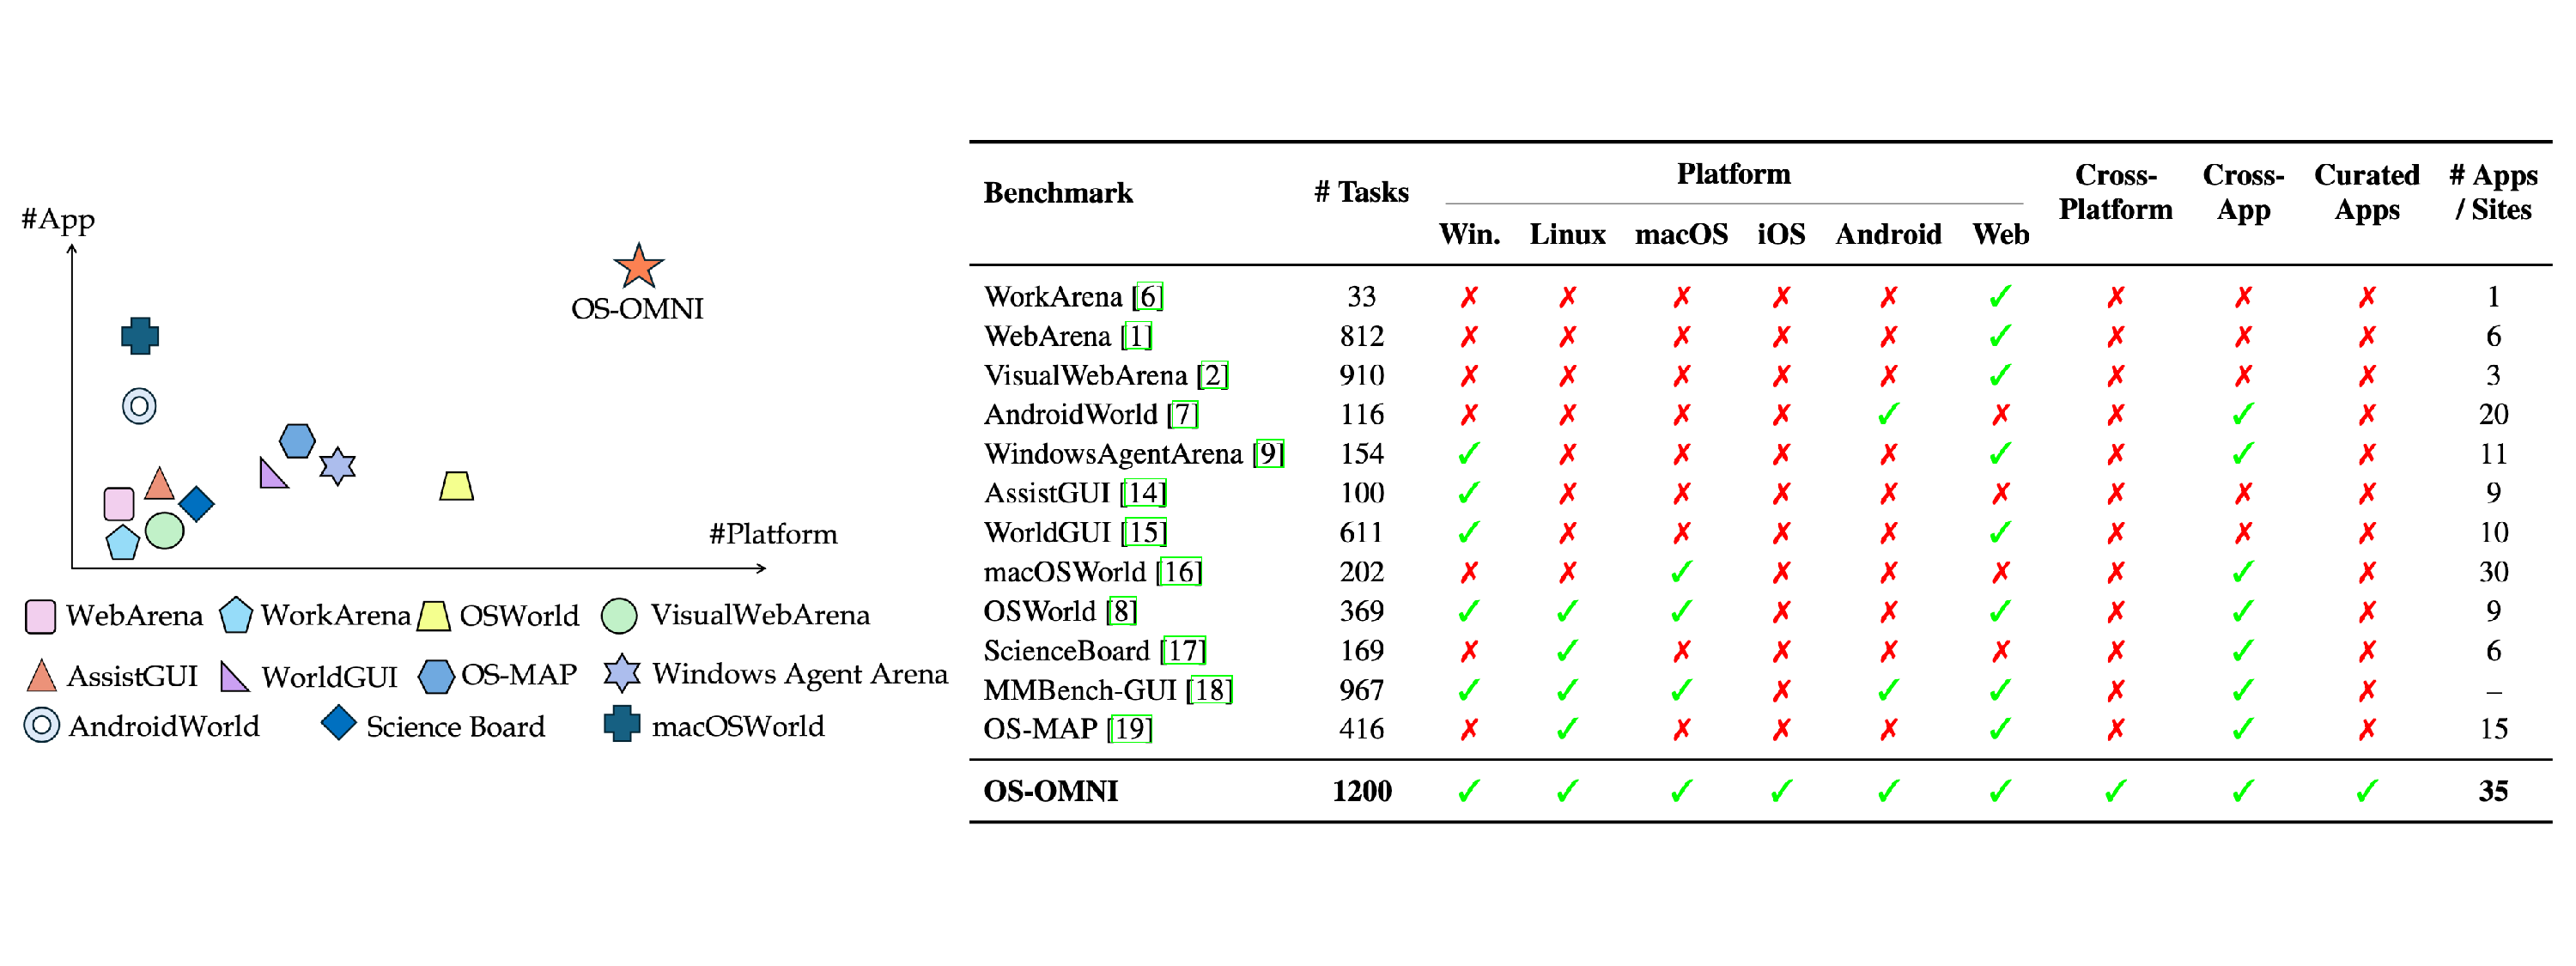
\includegraphics[width=1\textwidth]{figures/table1.pdf}
    }
    \vspace{-3em}
    \caption{
\#Platform indicates the number of supported platforms among Windows, Linux, macOS, iOS, Android, and Web, and \#App indicates the number of covered applications or websites. 
% For task properties, Cross-Platform denotes workflows spanning multiple operating systems or runtime environments, Cross-App denotes coordination across multiple applications, and Curated Apps denotes benchmark-controlled applications or services with reproducible account or service state and final-state evaluation. 
Compared with existing benchmarks, \dataset provides broader platform coverage, richer application diversity, cross-platform workflows, and curated application.
}
    \vspace{-15pt}
    \label{fig:comparison_benchmarks}
\end{figure}

\subsection{Observation Space}
\label{observation_space}
% \dataset supports three observation modes, selected by the execution specification: screenshot-only, accessibility tree-only, and combined observation. Screenshots provide the most uniform observation across platforms and are available for all supported environments. Accessibility trees provide structured UI information when the underlying system exposes it. The combined mode records both modalities, allowing agents to use visual and structured information jointly. The benchmark does not assume that structured UI metadata is always complete or available. Since structured UI metadata can be incomplete, unavailable, or noisy, and recent GUI-agent systems~\citep{} increasingly rely on purely visual observations for generality and cross-platform transfer, all experiments reported in this paper use the screenshot-only observation mode unless otherwise stated.

\dataset supports three observation modes through the execution specification: screenshot-only, accessibility tree-only, and combined observation. We adopt screenshot-only observation as the main experimental setting because screenshots are available across all supported platforms and provide the most uniform interface for generalist computer-using agents. This choice is also aligned with the recent trend of vision-centric CUA agents, where agents increasingly operate from screenshots to improve generality across heterogeneous applications and operating systems~\citep{cheng2024seeclick,wang2024mobile,lu2024omniparser,lin2025showui}. 
% citation required
Accessibility trees, while useful when available, are platform- and application-dependent: their metadata can be incomplete or unavailable. Therefore, all experiments reported in this paper use screenshot-only observation unless otherwise stated. At the same time, \dataset also supports accessibility tree-only and combined observation modes, enabling future studies to evaluate agents that rely on structured UI metadata or combine visual and accessibility-based information.

\subsection{Action Space}
\label{action_space}

% \begin{wraptable}{r}{8cm}
% \vspace{-5pt}
% \caption{Examples of actions supported by \dataset, see App.~\ref{} for the complete list. Platform adapters translate the shared action intent into native desktop or mobile control commands.}
% \centering
% \resizebox{1.0\linewidth}{!}{%
% \begin{tabular}{@{}ll@{}}
% \toprule
% Function & Description \\
% \midrule
% \texttt{click(x, y)} & Selects a coordinate on the current screen. \\
% \texttt{double\_click(x, y)} & Sends two consecutive clicks where supported. \\
% \texttt{write(`text')} & Enters text into the focused field. \\
% \texttt{press(`enter')} & Sends one keyboard key. \\
% \texttt{hotkey(`ctrl', `s')} & Sends a key combination. \\
% \texttt{scroll(delta)} & Scrolls the active view. \\
% \texttt{dragTo(x, y)} & Performs a pointer drag. \\
% \texttt{swipe(x1, y1, x2, y2)} & Performs a touch-style swipe. \\
% \texttt{WAIT} & Gives the interface time to update. \\
% \texttt{FAIL} & Declares that the task cannot be completed. \\
% \texttt{DONE} & Declares that the task is complete. \\
% \bottomrule
% \end{tabular}
% }
% \vspace{-0.1in}
% \label{tab:pyautogui_examples}
% \end{wraptable}

In \dataset, we introduce a two-level action space that combines a basic, platform-agnostic action interface with customized platform execution. The basic layer covers common human-computer operations, including pointer actions, keyboard shortcuts, text entry, scrolling, dragging, touch-style gestures, waiting, and terminal decisions \texttt{DONE} and \texttt{FAIL}. This layer follows the widely used PyAutoGUI-style semantics for mouse and keyboard control, making the agent-facing syntax compact and familiar. The customized layer maps each high-level action intent to the most reliable native backend available on each endpoint. For example, a \texttt{click} action may be executed as a PyAutoGUI desktop event on Linux, a Windows or macOS runtime call, an ADB tap on Android, or an Appium/XCUITest action on iOS. This separation between action syntax and execution backend allows \dataset to evaluate agents under a shared interface without forcing heterogeneous operating systems to expose the same automation API. As a result, the action space is broad enough to cover realistic GUI workflows across desktop and mobile platforms, while remaining structured enough for cross-platform comparison. We show complete action lists in Appendix~\ref{app:osomni_action}.


% We show actions examples in Appendix~\ref{}. Following the previous work, we use the widely used mouse and keyboard control library pyautogui for our action space. The design deliberately separates action syntax from execution backend. A click may become a pyautogui-like desktop event, a Windows or macOS runtime call, an ADB tap, or an Appium action depending on the platform. This keeps the agent-facing interface stable while allowing each runtime to use the most reliable native control channel. The resulting action space is broad enough for realistic GUI operation but constrained enough to log and replay.


% The customized layer maps each high-level action intent to the most reliable
% native backend available on each endpoint. For example, a \texttt{click} action
% may be executed as a PyAutoGUI-like desktop event on Linux, a Windows or macOS
% runtime call, an ADB tap on Android, or an Appium/XCUITest action on iOS. This
% separation between action syntax and execution backend allows \dataset to
% evaluate agents under a shared interface without forcing heterogeneous operating
% systems to expose the same automation API. As a result, the action space is
% broad enough to cover realistic GUI workflows across desktop and mobile
% platforms, while remaining structured enough for validation, logging, replay,
% and cross-platform comparison.